
\subsection{Introduction}
Lithium-ion batteries packs large amounts of energy in a small package and can power systems for long periods before a recharge is needed. Because of the high energy density they have to be handled with care. Beyond protection a \gls{bms} can be used to report battery percentages and remaining capacity. The specific type of battery used in this project is ICR18650.


\subsection{Lithium-ion Battery Composition}
Lithium-ion batteries are similar to other batteries in the way that they work by the same electrochemical principles. Though there are differences that has to be taken into account when developing a battery management system.

A lithium-based battery does not have any metallic lithium in it, instead, lithium ions are intercalated in the electrode material. Due to the highly reversible properties of the intercalation, \gls{lion} have greater electrode stability and cycle life compared to other electrochemical processes. They have high coulombic efficiency in all states of charge. Self-discharge is also slower in \gls{lion} batteries which makes them useful in situations where they may not be used for extended periods and are expected to work once the system turns on.

Memory effects present in other chemistries which causes gradual loss of capacity if not discharged properly are not present in lithium-ion batteries and makes the usage more flexible. Trickle charging is a common method of determining the \gls{soc}, but lithium-ion batteries lead to overcharging and may damage the batteries.

Water-based electrolytes are common in most batteries but as electrolysis begins at two volts in water and the voltages present in lithium cells are higher than that, that is not possible. Organic solvents are instead used. These solvents are flammable and have high vapour pressures. The increased performance of \gls{lion} batteries comes with higher severity if something would go wrong, so they have to be handled with extra care.

One of the most common form factors is the cylindrical cell referred to as 18650. That is $18mm$ in diameter and $65mm$ in length \cite[p. 26-27]{book}. The figure \autoref{fig:cellstruct} displays the parts that build up such a cylindrical cell.

\begin{figure}[H]
	\centering
	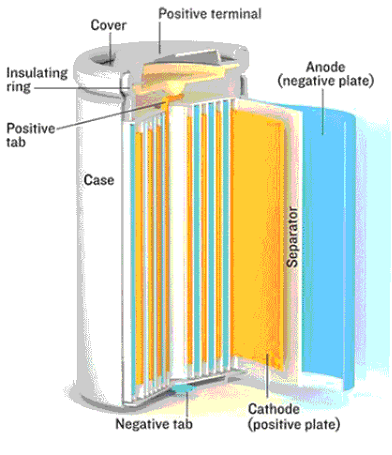
\includegraphics[width=0.3\textwidth]{Figures/cellstruct.png}
	\caption{\gls{lion} 18650 battery structure.}
	\label{fig:cellstruct}
\end{figure}

\subsection{Charging}

Charging can be either controlled by a separate charger or by the management system itself. Whichever implementation is used, these are the tasks the battery management system must perform\cite[p.111]{book}:

\begin{itemize}[noitemsep]
	\item Charging rate
	\item Life of the batteries
	\item Charge termination
\end{itemize}

The preferred way of charging \gls{lion} batteries is \gls{cccv}-charging. The charge cycle begins with a constant current after the specification of the battery in use. This current is supplied continually until the battery has reached its end-of-charge-voltage. Then charging is switched over to constant voltage mode and the current will taper off as the cell reaches its full capacity. Charging is then terminated when the current goes below a predefined value. \autoref{fig:cccv} displays the process\cite{cccv}. As the voltage curve is steep when the battery reaches its full capacity precise regulation is needed to prevent overcharging\cite[p.111-112]{book}.

\begin{figure}[H]
	\centering
	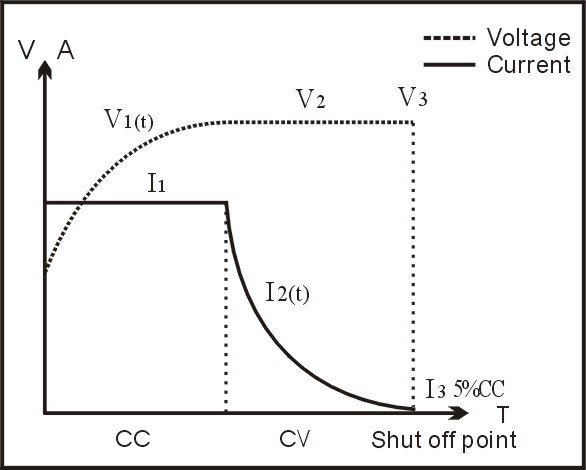
\includegraphics[width=0.45\textwidth]{Figures/cccv.jpg}
	\caption{Behaviour of \gls{cccv}-charging.}
	\label{fig:cccv}
\end{figure}

\subsection{Balancing}
Unlike other types of batteries that have a lower coulombic efficiency, lithium-ion batteries do not self-balance during a charge cycle. Without the ability to transfer charge, capacity will be limited to the battery with the lowest capacity in a series configuration. Knowing the capacity in real-time increases the efficiency of the balancing process.
Cell balancing is used for one or more of these purposes\cite[p.183-185]{book}:
\begin{itemize}[noitemsep]
	\item Minimize charge difference
	\item Maximize available battery power
	\item Maximize available battery energy
\end{itemize}
\autoref{fig:variations} Shows the variations that can occur between cells in a series stack.
\begin{figure}[H]
	\centering
	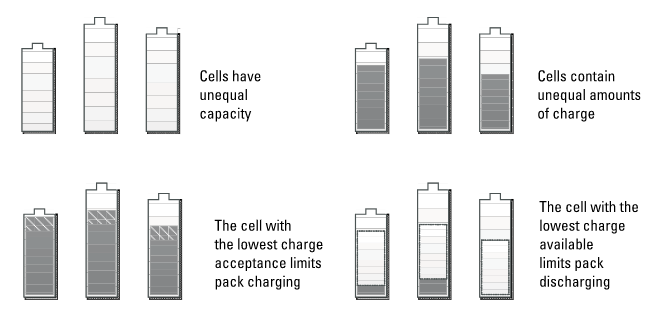
\includegraphics[width=0.8\textwidth]{Figures/variations.png} 
	\caption{Series stack cell variations.}
	\label{fig:variations}
\end{figure}

\subsection{18650 Basic Safety}
There are both protected and unprotected 18650 batteries. Protected ones include three basic safety features\cite{webpage}:

\begin{itemize}[noitemsep]
	\item \gls{ptc}
	\item \gls{cid}
	\item \gls{pcb}
\end{itemize}

A \gls{ptc} is a resistor that increases resistance when temperature rises, thus protecting against over temperatures. It will automatically reset when the temperature goes down.
\gls{cid} or pressure valve disables the battery permanently if the vapor pressure inside the cell becomes too high. Preventing further swelling and possible fire.
The \gls{pcb} protects against over discharge, overcharge, and overcurrent. Depending on the design, it will be reset when there is no fault condition any more or when it is placed in a charger.  

\autoref{fig:protection} is an illustration of a protected \gls{lion} battery. The pressure valve on the left side also breaks the connection between the internal and external positive pole which is why it is called \gls{cid} or current interrupt device.

\begin{figure}[H]
	\centering
	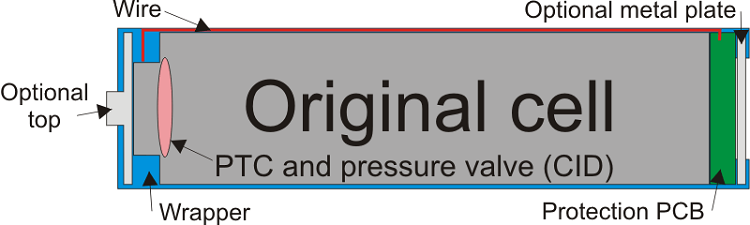
\includegraphics[width=0.45\textwidth]{Figures/protection.png}
	\caption{A protected 18650 cell.}
	\label{fig:protection}
\end{figure}

\subsection{Safety and Abuse Conditions}

Due to the differences between \gls{lion} batteries and other batteries, their higher capacity makes them more susceptible to faults when abused. A list of abuse conditions and their implications follows\cite[p.35-38]{book}.

\begin{itemize}
\item Overcharge occurs when \gls{soc} is greater than $100\%$. Cell voltage will begin to rise fast and may damage load or monitoring circuitry. Irreversible degradation inside the cell will occur. Both single large events and many small events cause degradation. Unlike in other chemistries, small currents causes this. Leading to thermal runaway, cell swelling, and venting. Begins somewhere between $3.75V$ and $4.2V$ depending on the cell.
\item Over-discharge occurs when \gls{soc} reaches below $0\%$, the voltage decreases fast and can even be reversed if discharge current is too high. A reversed voltage may result in damaged monitoring circuitry. Internal damage includes dissolution of the negative terminal foil. Self-over-discharge cannot be prevented. Minimum voltage before over discharge occurs is between $1.8-2.5V$ depending on the cell.
\item High temperatures increase cell degradation which in turn causes thermal runaway further increasing inside temperatures. Excessive temperatures activate exothermic chemical reactions in the organic solvents. Releasing high amounts of energy that leads to venting of cell contents, fire or explosion.
\item Low temperatures can cause plating of metal lithium onto the electrodes which leads to irreversible capacity loss and possibly metallic ``dendrite'' growth. Dendrites can penetrate the separator leading to internal short circuits. Low temperatures also increase cell impedance thus limiting discharging capabilities. Charging below $0\degree C$ is not recommended, although some cells allow temperatures below $-10\degree C$.
\item Overcurrent, both during dis- and re-charging can cause the same type of problems as with general over- and under-charge conditions, at the same time high currents increases temperature. The maximum current allowed for is a function of \gls{soc} and temperature. Even though temperature would be held at acceptable levels, the amount of current will still be limited by the number of ions the negative terminal can receive at any given moment.
\item Age is a major factor when it comes to Li-ion batteries, the risk of failure increases with age. Monitoring and estimating remaining battery lifetime can be done and is expressed in \gls{soh}.
\end{itemize}

\subsection{Determining \gls{bms} Specifications}
A flow chart was used to determine the power requirements of the system powered by the batteries. As is seen in \autoref{fig:powerinput}. The particular \gls{mcu} runs on $3.3V$ and the sensors that were chosen runs on $3.3V$ and $5.5V$ respectively, so those requirements where definite. There were thoughts about adding a display that might have needed $12V$, therefore the light blue block in \autoref{fig:powerinput}. As the project continued it was omitted and $12V$ would not be needed. Therefore two batteries in series are used. Resulting in a voltage range of $8.4V$ fully charged and down to $6V$ fully depleted. This voltage is stepped down to $5V$ and supplied to the system.
Current wise it was not known how much the system would draw but it was estimated that the capacity of the batteries of $2.2Ah$ would be enough to power the system for several hours.
In a worst-case scenario, the system would draw more than $500mA$ which would result in $4h$ and $24min$ of usage.
Safety is of high priority as concluded earlier. So a second flowchart was created to determine the specifications of the monitoring of the two batteries in a series configuration. \autoref{fig:battery} displays these specifications.

\begin{figure}[H]
	\centering
	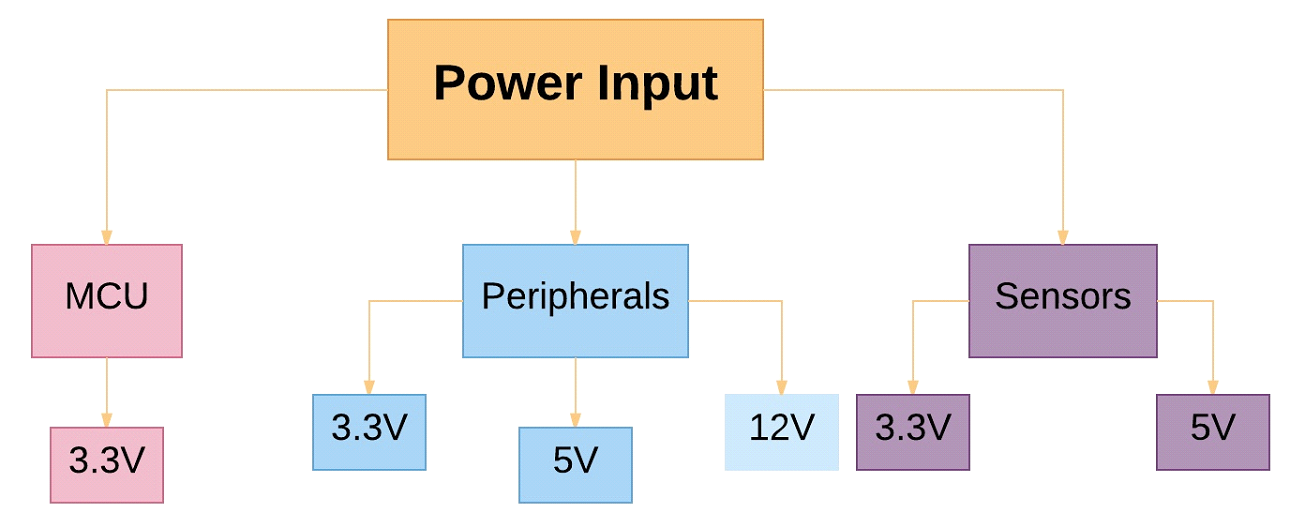
\includegraphics[width=\textwidth]{Figures/powerinput.png}
	\caption{Power input flowchart.}
	\label{fig:powerinput}
\end{figure}

\begin{figure}[H]
	\centering
	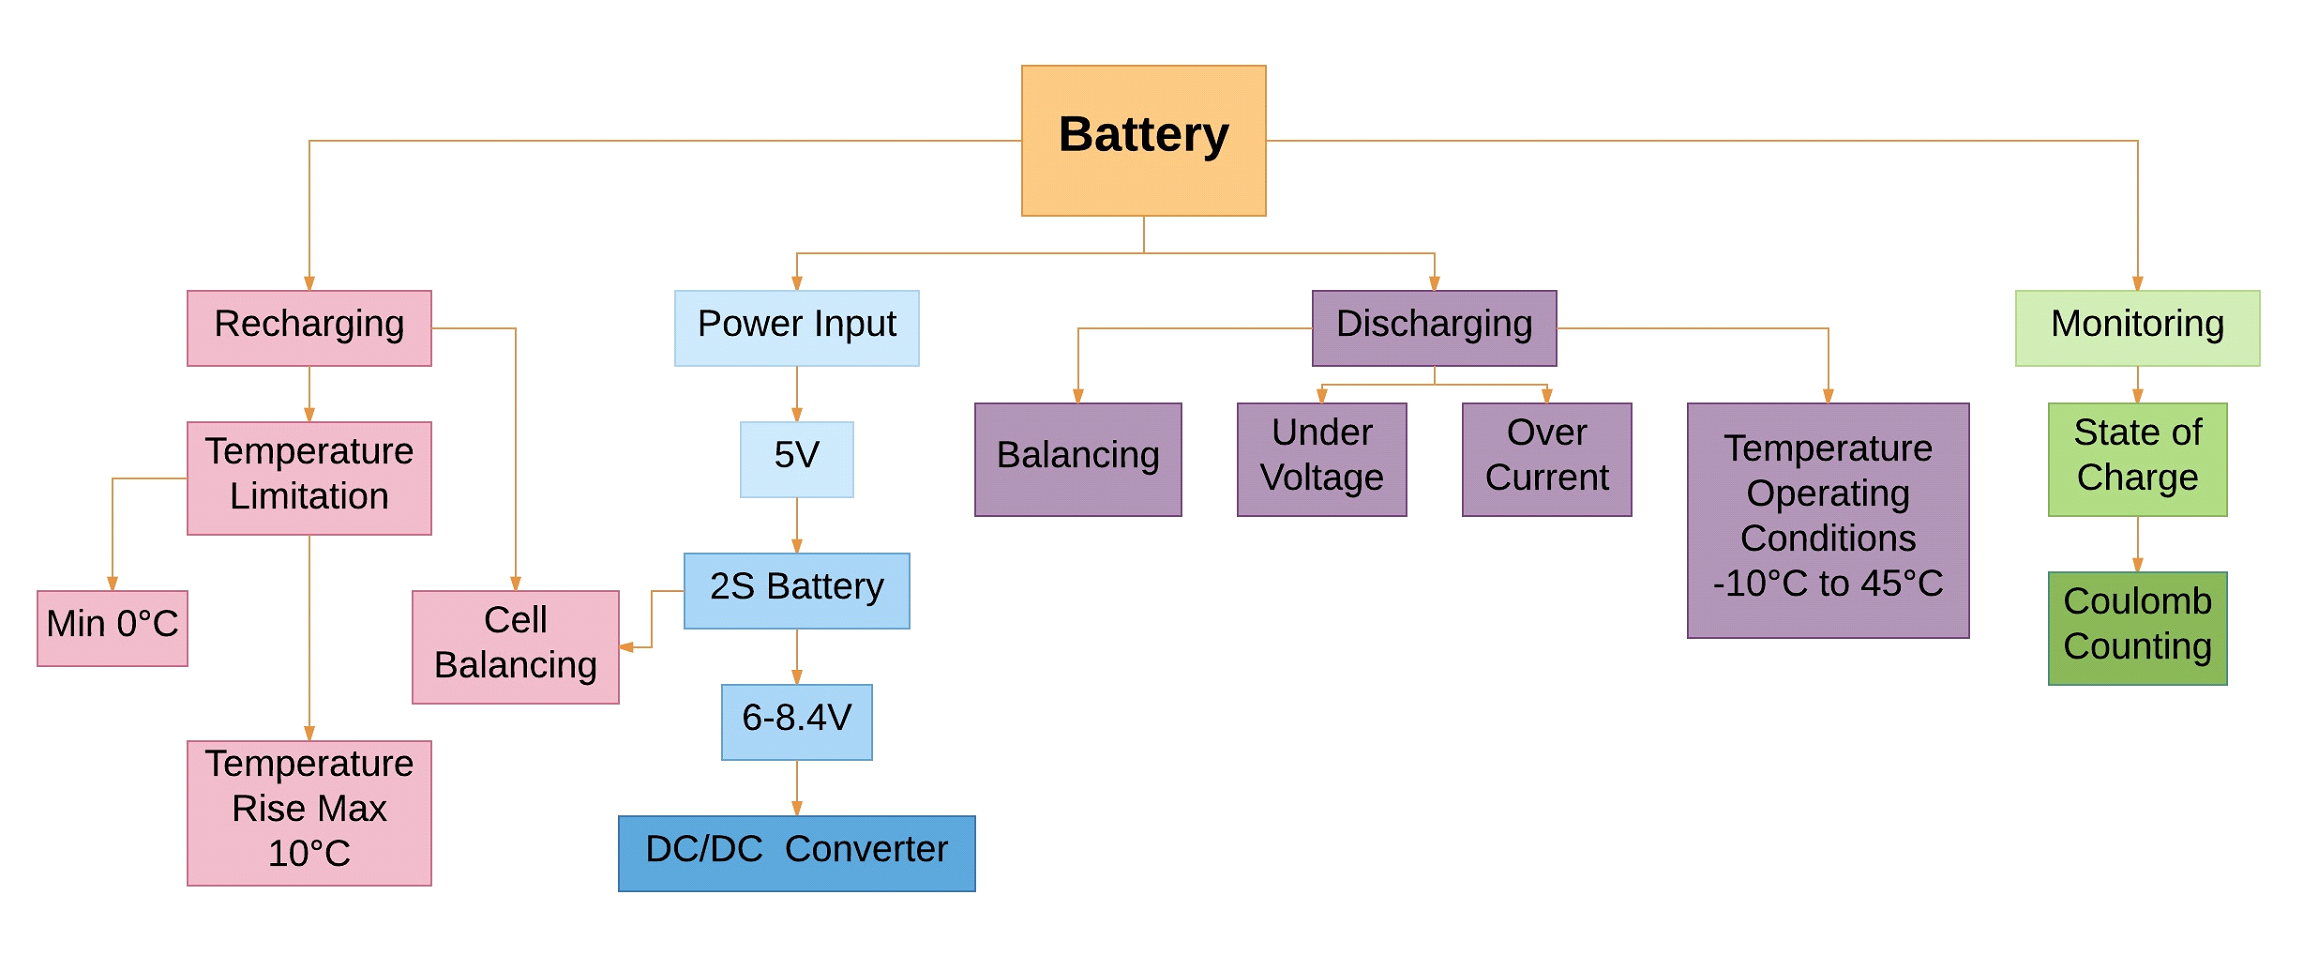
\includegraphics[width=\textwidth]{Figures/battery.png}
	\caption{Battery management flowchart.}
	\label{fig:battery}
\end{figure}


Three \gls{ic}s where chosen for the \gls{bms}. The BQ28Z610 is a gas gauge \gls{ic} for Li-ion batteries from \gls{ti}, including these features:

\begin{itemize}[noitemsep]
	\item \gls{i2c} communication of status to host.
	\item Balancing of cells, both during charge and use.
	\item Temperature monitoring and regulation.
	\item Under and overvoltage protection.
	\item Overcurrent protection.
	\item \gls{soc} reporting.
\end{itemize}

The BQ24133, also a \gls{ti} \gls{ic}, is chosen for charging purposes, making use of the following features:

\begin{itemize}[noitemsep]
	\item 1-3 series cells.
	\item Temperature monitoring and regulation.
	\item Power Path, load can safely be connected during charging.
\end{itemize}

The output voltage is managed by the \gls{ti} \gls{ic} LM2596 step-down converter.

During development, a BQ28Z610 development board was used together with a Luxorparts variable voltage regulator utilizing the LM2596 and a generic \gls{lion} \gls{2s} charger.

The BQ28Z610's software was configured using a windows computer, \gls{ti}'s software bqStudio\cite{bqStudio} and the EV2300 \gls{pc} interface board.
A \gls{pwb} containing the three \gls{ic}'s mentioned above was designed using KiCad\cite{kicad}. The designs were made according to the typical application of each \gls{ic}. Typical applications are found in data sheets.  

\subsection{Current State}
\autoref{fig:modules} displays how the \gls{bms} is currently set up. Up left on top of the main PCB is the BQ28Z610 development board, and below that is the voltage regulator. Charging is enabled via the charging port visible to the right, on the lid.

\begin{figure}[H]
	\centering
	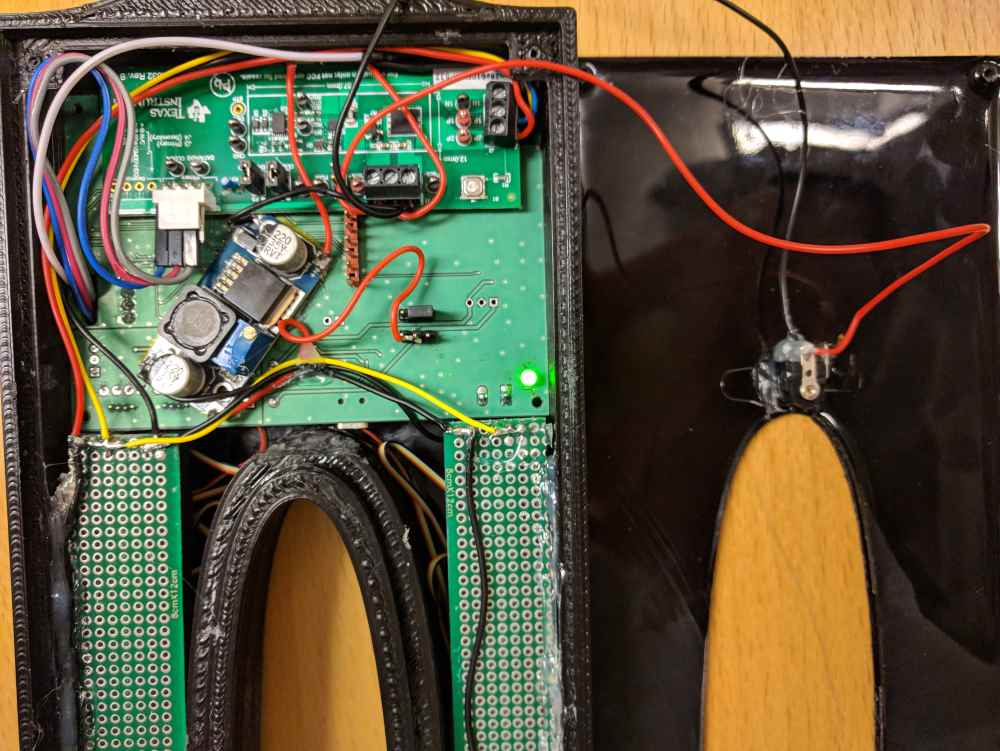
\includegraphics[width=0.6\textwidth]{Figures/modules.png}
	\caption{Current setup of the battery management.}
	\label{fig:modules}
\end{figure}


Charging is done by turning the device upside down and connecting a \gls{2s} \gls{lion} charger. See\autoref{fig:charging}.

\begin{figure}[H]
	\centering
	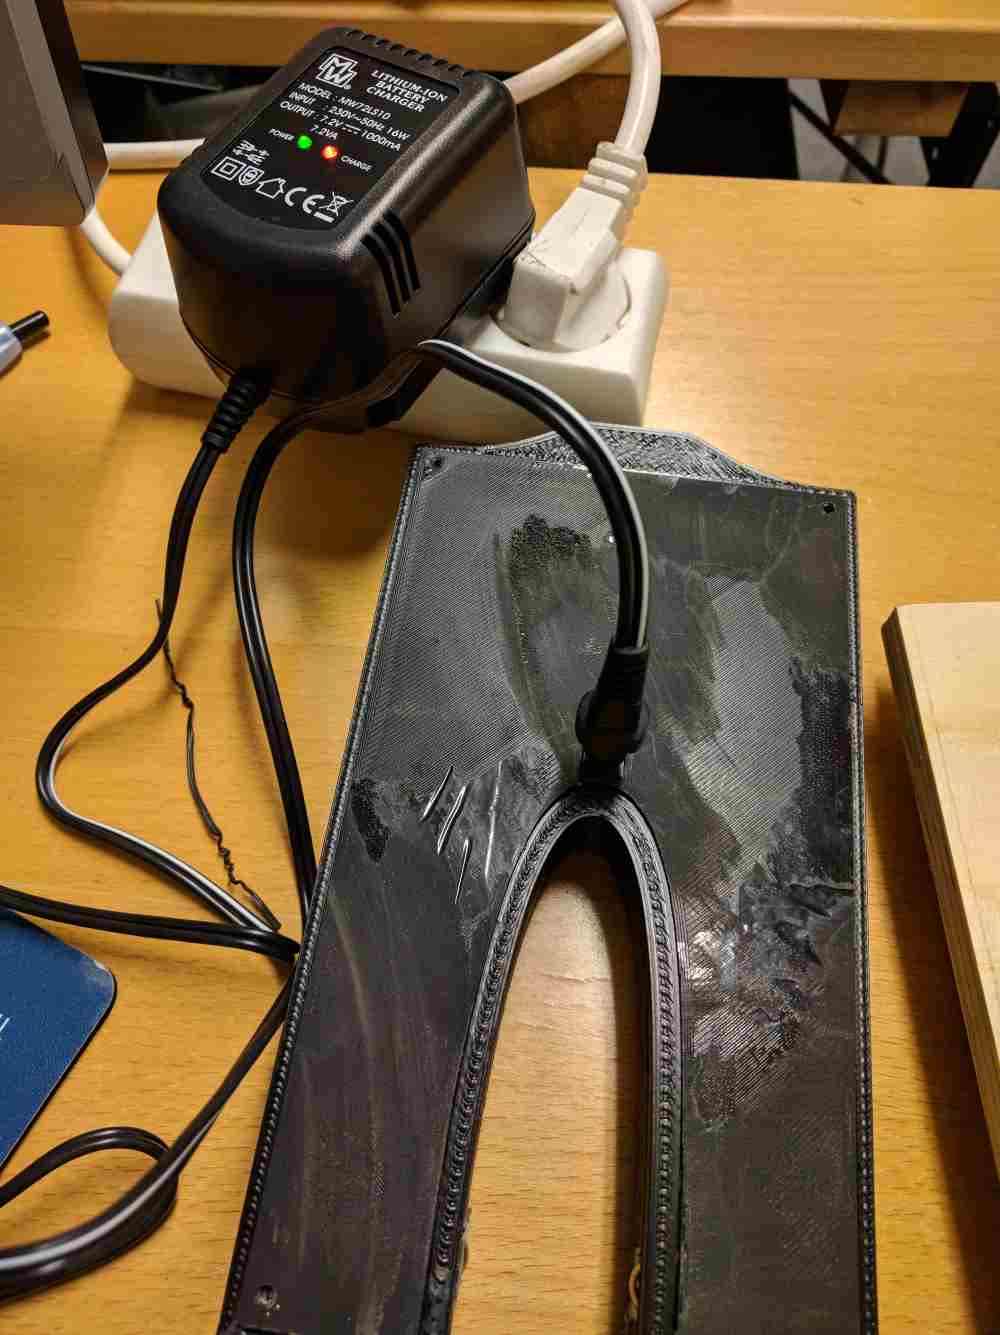
\includegraphics[width=0.45\textwidth]{Figures/charging.png}
	\caption{How to charge.}
	\label{fig:charging}
\end{figure}

A connection diagram for this configuration can be seen in \autoref{fig:diagram}. The charger is connected to the input of the voltage regulator. This configuration has all the features of that implemented on the \gls{pwb} except the charger is external, charges with $1A$ instead of $2A$ and there is no power path, meaning that the device has to be turned off to make charging safely.

\begin{figure}[H]
	\centering
	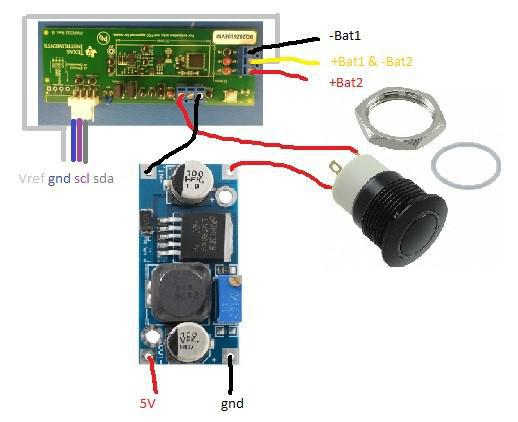
\includegraphics[width=0.6\textwidth]{Figures/diagram.jpg}
	\caption{Connection diagram.}
	\label{fig:diagram}
\end{figure} 

\autoref{fig:bmspwb} shows the \gls{pwb} that when soldered and tested would fulfill all requirements. It is supposed to be the entire \gls{bms}. 
Schematics, board layout, and Gerber-files can all be found in the appendix. %Nope. Not there. Also, refer to them!: Can be found in the appendix, see: \autoref{first}, \ref{second}, ..., and \ref{last}.

\begin{figure}[H]
	\centering
	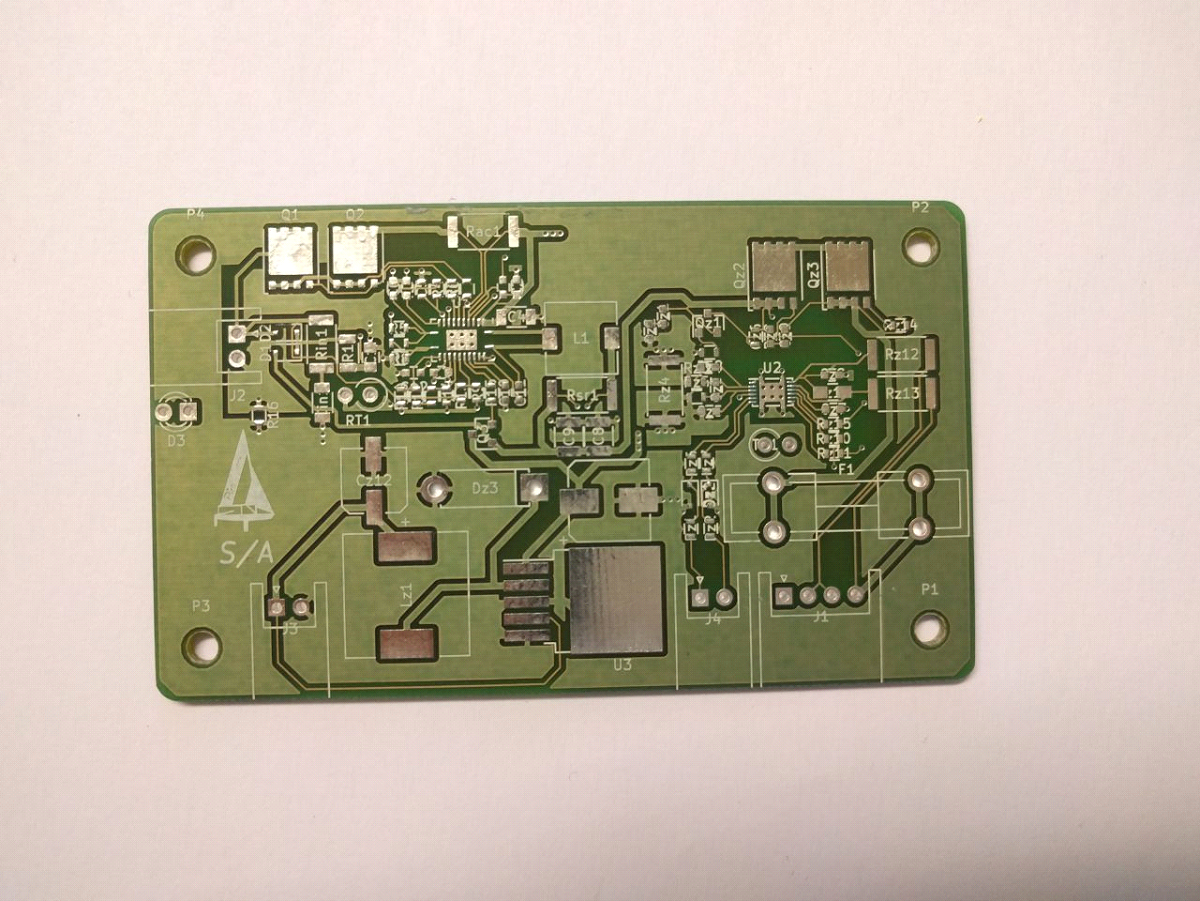
\includegraphics[width=.6\textwidth]{Figures/bmspwb.png}
	\caption{Battery management \gls{pwb}.}
	\label{fig:bmspwb}
\end{figure}
